\chapter{Παράρτημα Α - Δείγματα εικόνων}

\DeclareGraphicsExtensions{.pdf,.png,.jpg}
\graphicspath{{appendix1/fig/}}

\begin{figure} 
\centering 
%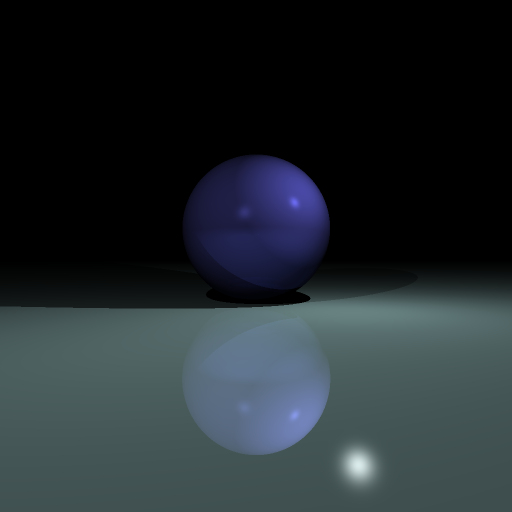
\includegraphics[width=90mm, height=90mm, keepaspectratio=true]{scn_sphere}
\caption{H σκηνή sphere}
\end{figure}

\begin{figure} 
\centering 
%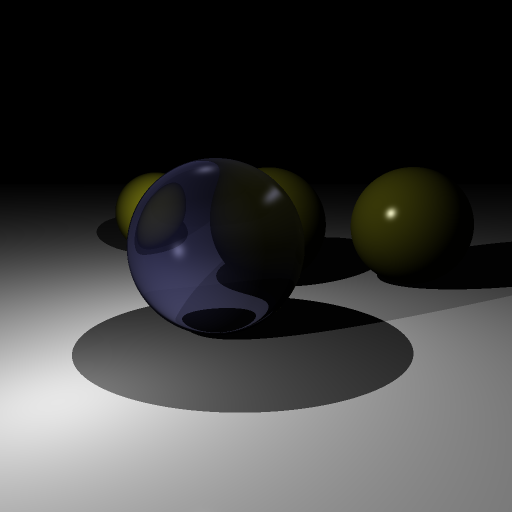
\includegraphics[width=90mm, height=90mm, keepaspectratio=true]{scn_refraction}
\caption{H σκηνή refraction}
\end{figure}

\begin{figure} 
\centering 
%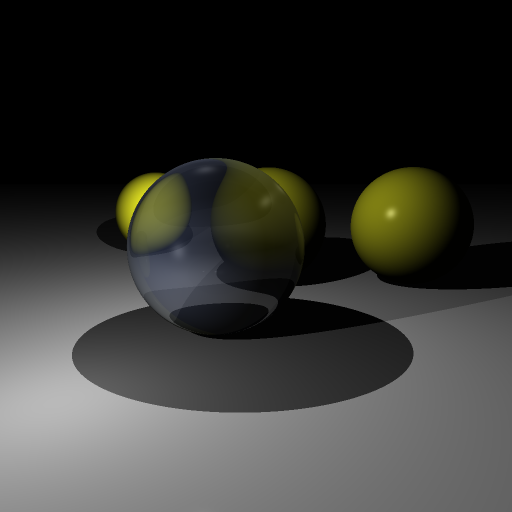
\includegraphics[width=90mm, height=90mm, keepaspectratio=true]{scn_refraction_1033}
\caption{H σκηνή refraction με διαφορετικό material}
\end{figure}

\begin{figure} 
\centering 
%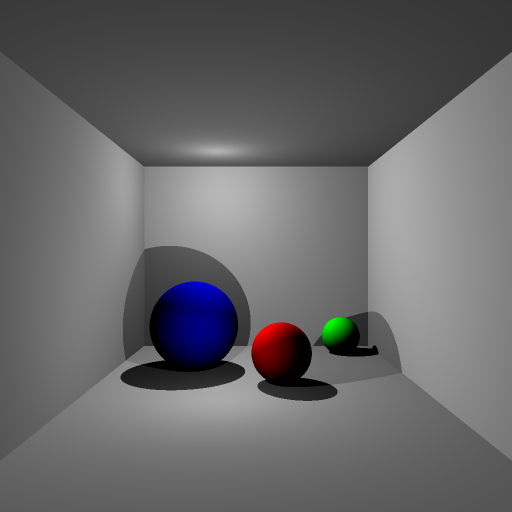
\includegraphics[width=90mm, height=90mm, keepaspectratio=true]{scn_room_lambert}
\caption{H σκηνή room lambert}
\end{figure}

\begin{figure} 
\centering 
%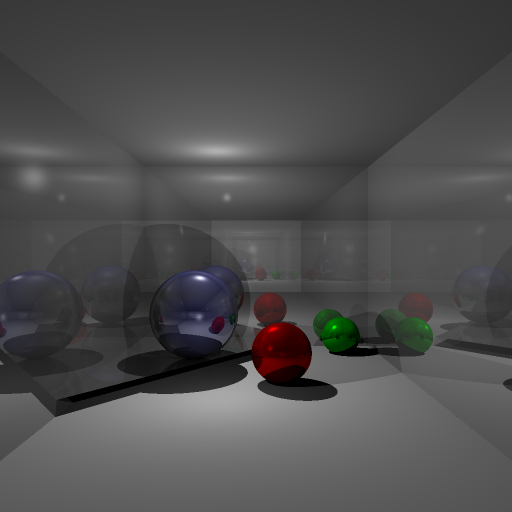
\includegraphics[width=90mm, height=90mm, keepaspectratio=true]{scn_room_phong}
\caption{H σκηνή room phong}
\end{figure}

\begin{figure} 
\centering 
%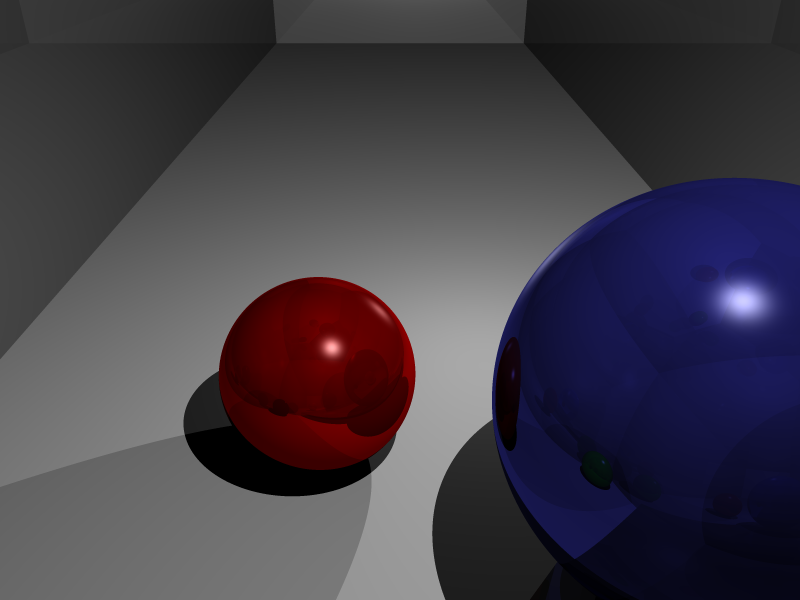
\includegraphics[width=90mm, keepaspectratio=true]{scn_room_2}
\caption{H σκηνή room phong από άλλη κάμερα}
\end{figure}

\begin{figure} 
\centering 
%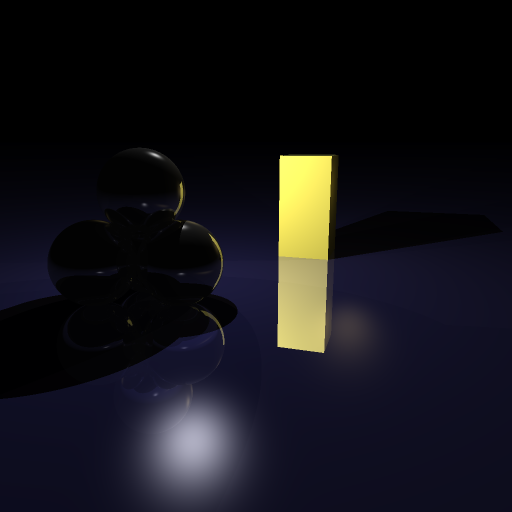
\includegraphics[width=90mm, height=90mm, keepaspectratio=true]{scn_trophy}
\caption{H σκηνή trophy}
\end{figure}

\begin{figure} 
\centering 
%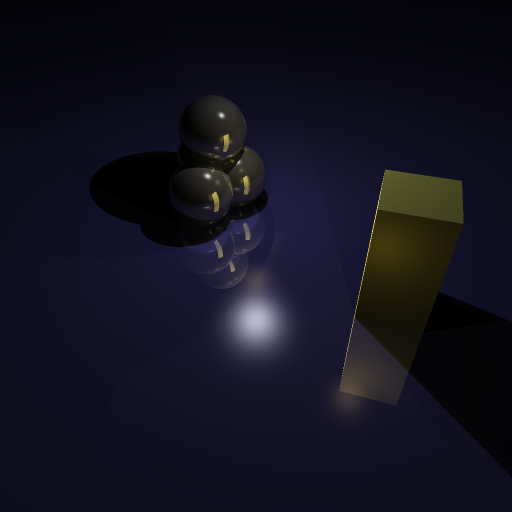
\includegraphics[width=90mm, height=90mm, keepaspectratio=true]{scn_trophy_2}
\caption{H σκηνή trophy από άλλη κάμερα}
\end{figure}

\begin{figure} 
\centering 
%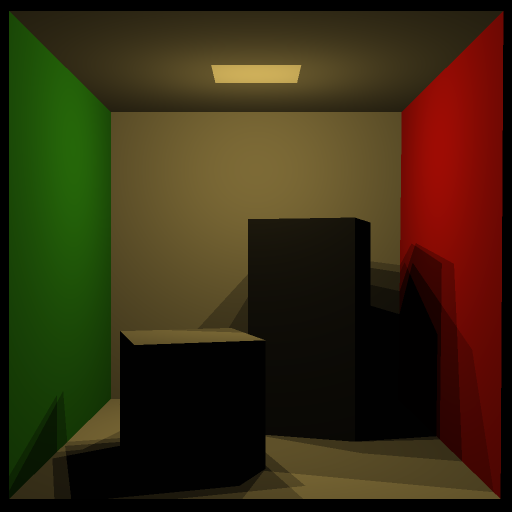
\includegraphics[width=90mm, height=90mm, keepaspectratio=true]{scn_cornell_box}
\caption{H σκηνή cornell box}
\end{figure}

\begin{figure} 
\centering 
%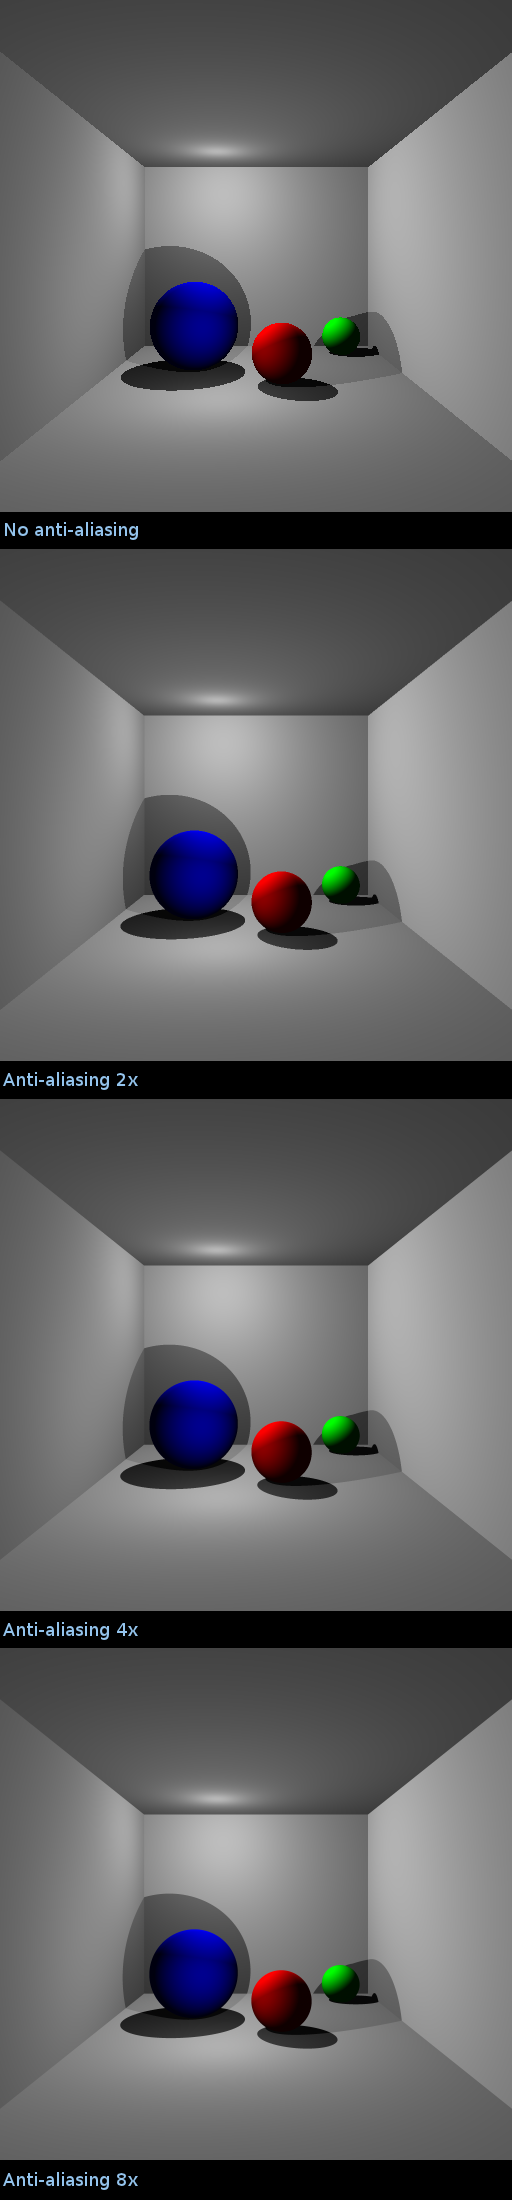
\includegraphics[width=40mm, keepaspectratio=true]{scn_antialiasing}
\caption{Antialiasing}
\end{figure}

\begin{figure} 
\centering 
%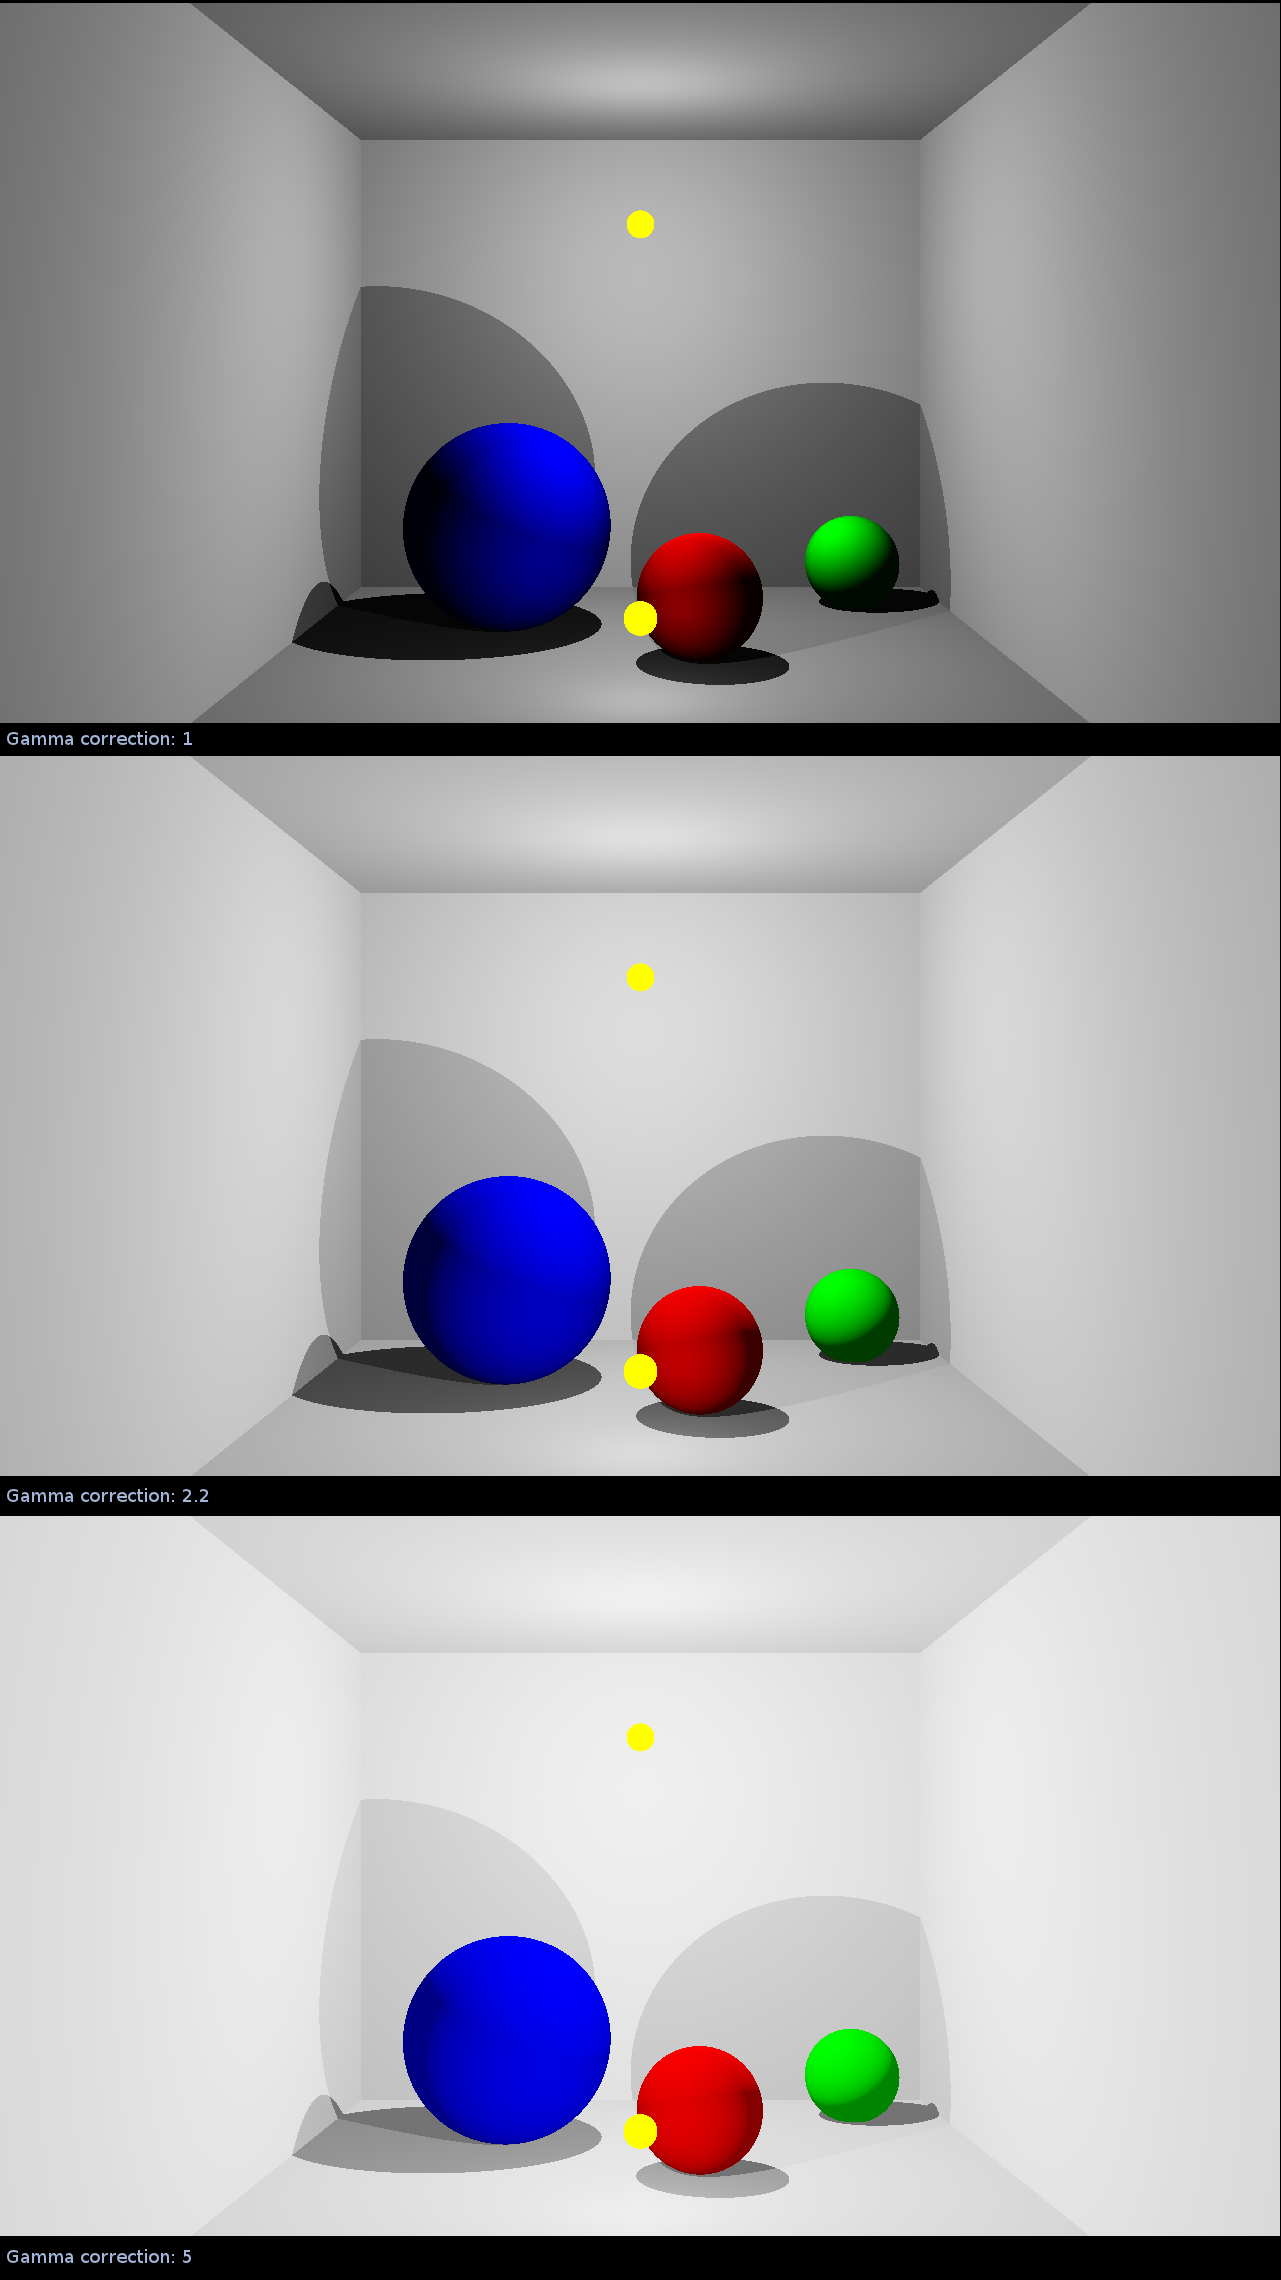
\includegraphics[width=70mm, keepaspectratio=true]{scn_gamma}
\caption{Gamma correction}
\end{figure}
